%%%%%%%%%%%%%%%%%%%%%%%%%%%%%%%%%%%%%%%%%
% University/School Laboratory Report
% LaTeX Template
% Version 3.1 (25/3/14)
%
% This template has been downloaded from:
% http://www.LaTeXTemplates.com
%
% Original author:
% Linux and Unix Users Group at Virginia Tech Wiki 
% (https://vtluug.org/wiki/Example_LaTeX_chem_lab_report)
%
% License:
% CC BY-NC-SA 3.0 (http://creativecommons.org/licenses/by-nc-sa/3.0/)
%
%%%%%%%%%%%%%%%%%%%%%%%%%%%%%%%%%%%%%%%%%

%----------------------------------------------------------------------------------------
%	PACKAGES AND DOCUMENT CONFIGURATIONS
%----------------------------------------------------------------------------------------

\documentclass{article}

\usepackage[version=3]{mhchem} % Package for chemical equation typesetting
\usepackage{siunitx} % Provides the \SI{}{} and \si{} command for typesetting SI units
\usepackage{graphicx} % Required for the inclusion of images
\usepackage{natbib} % Required to change bibliography style to APA
\usepackage{amsmath} % Required for some math elements 
\usepackage[utf8]{inputenc}
\usepackage{algorithm}
\usepackage{algpseudocode}
\usepackage{authblk}
\usepackage{amssymb}
\usepackage[spanish]{babel}
\usepackage{url}
\usepackage{listings}
\usepackage[toc,page]{appendix}
\usepackage{booktabs}

\setlength\parindent{0pt} % Removes all indentation from paragraphs

\renewcommand{\labelenumi}{\alph{enumi}.} % Make numbering in the enumerate environment by letter rather than number (e.g. section 6)

%\usepackage{times} % Uncomment to use the Times New Roman font

%----------------------------------------------------------------------------------------
%	DOCUMENT INFORMATION
%----------------------------------------------------------------------------------------

\title{Obligatorio 1 \\ Métodos Númericos 2015 } % Title

\author{Matías \textsc{Estrada} | 3.858.107-2 | estrada.matias@gmail.com
\and Gonzalo \textsc{Javiel} | 4.666.259-5 | gonzalo.javiel@gmail.com
\and Andrés \textsc{Tipoldi} | 3.834.437-9 | tipoldi@gmail.com
\and Raúl \textsc{Speroni} | 4.177.047-8 | raulsperoni@gmail.com } % Author name

%\date{\today} % Date for the report

\begin{document}


% --------
% CARATULA
% --------

\begin{titlepage}
\maketitle % Insert the title, author and date
\end{titlepage}
% If you wish to include an abstract, uncomment the lines below
% \begin{abstract}
% Abstract text
% \end{abstract}

\tableofcontents
\newpage

%----------------------------------------------------------------------------------------
%	SECTION 1
%----------------------------------------------------------------------------------------

\section{Fundamentos}

\subsection{Matriz de Google}
\label{definitions}

Se llama Matriz de Google a una matriz estocástica particular utilizada por el algoritmo \textit{PageRank} del buscador de la empresa Google.
\textit{PageRank} cuenta la cantidad y calidad de enlaces hacia una página para estimar la importancia de una página web, la hipótesis primordial es que las páginas más relevantes probablemente tengan mayor cantidad de enlaces hacia ellas.
La matriz de Google se puede representar como un grafo orientado, donde los nodos son páginas web y las aristas son enlaces entre páginas. \cite{2345160020060101}  El \textit{PageRank} de cada página puede ser calculado iterativamente a partir de la matriz de Google usando por ejemplo el método de las potencias, para que el método converja la matriz debe ser estocástica, irreducible y aperiódica.

\begin{description}
\item[Matriz de Adyacencias]

Sea $N$ la cantidad de páginas, se define $A$ matriz de adyacencias que representa la relación entre enlaces como sigue:

\begin{equation} \label{eq:A}
A_{i,j} =
\left\{
	\begin{array}{ll}
		1  & \mbox{si $j$ tiene un enlace hacia $i$}\\
		0 & \mbox{en otro caso } 
	\end{array}
\right.
\end{equation}

\item[Matriz de Markov]
A partir de $A$ se construye una matriz $S$ que correspondiente a las transiciones en una cadena de Markov \cite{10261393320130701}. Sea $k_j$ el número de enlaces salientes del nodo $i$ a todos los demás nodos:

\begin{equation} \label{eq:S}
S_{i,j} =
\left\{
	\begin{array}{ll}
		A_{i,j}/k_{j}  & \mbox{si $j$ tiene un enlace hacia $i$}\\
		0 & \mbox{en otro caso } 
	\end{array}
\right.
\end{equation}

Aquellas columnas $j$ cuyos valores son todos cero representan nodos sin enlaces salientes, dichos vectores son reemplazados por otro cuyos valores sean $\dfrac {1} {N}$.
Por construcción la suma de todos los elementos de cada columna $j$ es la unidad, por lo tanto $S$ está bien definida, pertenece a la clase de Cadenas de Markov y a la clase de operadores de Perron-Frobenius.

\item[Matriz de Google]

Se puede definir la matriz de Google como sigue:

\begin{equation} \label{eq:G}
G_{i,j} = \alpha S_{i,j} + (1-\alpha) \dfrac {1} {N}
\end{equation}

\end{description} 

\subsection{Cadenas de Markov}

\begin{description} 
\item[Proceso markoviano] Un proceso markoviano es un proceso estocástico en el cual su comportamiento y su evolución futura no depende más que del estado actual del proceso y no de sus estados pasados. 

\item[ Cadena de Markov] Las Cadenas de Markov son procesos markovianos de espacio de estado discreto. Se pueden separar en Cadenas de Markov de tiempo discreto y Cadenas de Markov de tiempo continuo.

Una cadena de Markov puede definirse como una secuencia de variables aleatorias discretas  $\{X_n , n\in N \}$ que poseen la siguiente propiedad 

\begin{equation} \label{eq:markov}
\begin{split}
P(X_{n+1} = e_{n+1} | X_0 =e_0,X_1 =e_1, \cdots ,X_n =e_n) = P(X_{n+1} = e_{n+1} |X_n =e_n),  \\
\forall n \in N,\forall e_0,e_1, \cdots, e_n,e_{n+1} \in E
\end{split}
\end{equation}

Esta propiedad se interpreta como la afirmación que la probabilidad (condicional) del proceso alcance el estado futuro $x_{n+1}$ dados los estados pasado1s $x_0, x_1, \cdots x_{n-1}$ y el estado actual $x_n$ es independiente de los estados pasados y depende solamente del estado presente $x_n$ (el pasado no influye en el futuro más que a través del presente).

\item[Cadena de Markov ergódica] Una cadena de Markov es ergódica cuando es irreductible y su espacio de estado es un conjunto de estados ergódicos, o sea que todos sus estados son son recurrente positivos y aperiódicos.

\item[Teorema de ergodicidad] Toda Cadena de Markov de tiempo continuo homogénea finita e irreductible es ergódica. Si la cadena es infinita, puede no ser ergódica (una condición suficiente para que una cadena irreductible sea ergódica es que los valores $v_i$ estén acotados superiormente).

\end{description}

\subsection{Teorema de Perron Frobenius}

% TODO Creo que queda asociarlo más con la matriz de transicion de google, o sea que el valor propio es 1, que todos los valores propios son menores o iguales a 1, y la suma de coordenadas del vector pi es 1

Dada una matriz cuadrada $A\in M_{n \times n}$ con entradas positivas $a_{i,i} \geqslant 0$ entonces, 
\begin{enumerate}
\item Existe un valor propio $\lambda > 0$ tal que $A v= \lambda v$, donde el vector propio correspondiente es $v > 0$ 
\item Ese valor propio es mayor en módulo que todos los valores propios asociados a $A$ .
\item Cualquier otro vector  propio positivo de $A$ es múltiplo de $v$.
\end{enumerate}

Por construcción la matriz de Google es positiva, por lo que según el teorema de Perron Forbenius el valor propio de mayor módulo y el vector propio asociado al mismo existen.

\subsection{Vector propio dominante de la matriz de Google}

\begin{equation} \label{eq:v1}
Gv_{1} = v_{1}
\end{equation}

Sea $v_{1}$ el vector propio asociado al valor propio $1$ que verifica la ecuación \ref{eq:v1}  la i-esima componente de $v_{1}$ representa la probabilidad de estar en la página $i$ en un determinado momento $n$ y por lo tanto  $v_{1}$ representa la distribución de probabilidad de las páginas en el momento $n$. El vector $v_{1}$ se denomina distribución estacionaria. Siendo que nos brinda la probabilidad de encontrarse en cada página $v_{1}$ puede usarse para ordenar las páginas de acuerdo a su probabilidad. Este es uno de los componentes fundamentales del motor de búsqueda de Google.

%----------------------------------------------------------------------------------------
%	SECTION 2
%----------------------------------------------------------------------------------------

\section{Puntuación de Sitios Web}

\label{puntuacion}

\subsection{Método de potencias}
\begin{description}


\label{sub:pot} 
\item[Métodos de la potencias] Es un método iterativo que calcula sucesivas aproximaciones a los autovectores y autovalores de una matriz.
El objetivo del método es, dada una matriz $ M_{NxN} $ calcular el valor propio dominante y un vector propio asociado.

Sean los valores propios $ |\lambda_1|, .. |\lambda_N| $ que verifican $ |\lambda_1| > |\lambda_2| > ... > |\lambda_N| $ y su vectores propios asociados $ v_1, v_2, ..., v_n $

Sea $ x^{(0)} = \alpha_1 v_1 + \alpha_2 v2 + \alpha_N v_n $  con $ \alpha_1 \neq 0 $

\begin{equation*}
  \left\lbrace
  \begin{array}{l}
     y^{(j+1)} =  Mx^{(j)} \\ \\
     c_{(j+1)} = \text{ componente dominante de } y^{(j+1)} \\ \\
     x^{(j+1)} =  (\frac{1}{c_{(j+1)}}) y^{(j+1)} \text{ Normalizado de } y^{(j+1)} \\
  \end{array}
  \right.
\end{equation*}

Entonces se cumple:

La sucesión de escalares $ {c_j} $ tiende al valor propio dominante $ \lambda_1 $

$$
\{c_j\} \to \lambda_1 , j=0 \dots n
$$

%$ c_1, c_2, \dots, c_j, \dots \to \lambda_1$ %TODO PONER TIENDE CON J-INFINITO

La sucesión de vectores  $ \{x^{(j)}\}$ tiende a un vector propio normalizado asociado a $ \lambda_1 $

$$
\{x^{(j)}\} \to v_1 , j = 0 \dots n
$$
% $ x^{(1)},x^{(2)},\dots,x^{(j)}, \dots, v_1 $ % TODO VER BIEN %COMO ESCRIBIRLO

\end{description}


\subsection{Sistema lineal de ecuaciones}
\label{sub:sis}
\begin{equation} \label{eq:SLi}
Gv = \lambda v
\end{equation}
\begin{equation} \label{eq:SL}
(G-\lambda)v = 0
\end{equation}





\begin{description}
\item[Subespacio Krylov] Un subespacio de Krylov de orden $r$ generado por una matriz $A \in M_{NxN}$ y un vector $v$, es el subespacio vectorial generado por $A^{k}v$ con $k < r$:
\begin{equation} \label{eq:KY}
K_{r}(A,v) = span(v,Av,\ldots,A^{r-1}v)
\end{equation}

\item[Matriz de Hassenberg superior] Una matriz de Hassenberg superior tiene todos ceros por debajo de la primera subdiagonal.

 
\item[Método de Arnoldi] El método Arnoldi puede ser usado para encontrar todos los valores y vectores propios de la matriz $G \in M_{NxN}$, pertenece a la clase de algoritmos de álgebra lineal que producen un resultado parcial después de un número relativamente bajo de iteraciones. El algoritmo fue creado en principio para tranformar una matriz en forma Hassenberg superior, pero se encontró más adelante que el método podía ser usado para encontrar valores y vectores propios para matrices esparsas de gran tamaño de forma iterativa. Inicialmente el método construye bases del subespacio Krylov, después de construido el subespacio, con $m$ elegido como cantidad de bases, podemos calcular aproximaciones a los valores y vectores propios de la matriz esparsa original $G$. La matriz de Hassenberg $H \in M_{NxN}$ resultante del método es la clave para calcular esas aproximaciones ya que sus valores propios asociados $\lambda _{i}^{(m)}$ conocidos como \textit{Valores de Ritz} convergerán hacia los valores propios de la matriz esparsa de gran tamaño $A$ \cite{andersson2004investigating}.

Los vectores propios de la matriz de Google $G$ pueden calcularse como sigue:

\begin{enumerate}
  \item Calcular el valor propio de interés de $H$
  \item Obtener el vector propio asociado a ese valor propio.
  \item El vector correspondiente de $G$ se obtiene por:
  \begin{equation} \label{eq:GG}
	v_{i}^{(m)} = V_{m}y_{i}^{(m)}
\end{equation}
donde $v_{i}^{(m)}$ es el vector buscado en $G$, $V_{m}$ es el vector con bases del subespacio de Krylov y $y_{i}^{(m)}$ es el vector propio de $H$ asociado al valor propio de interés.   
  
\end{enumerate}

\item[Sistema Alternativo] la ecuación \ref{eq:G} determina una matriz $G$ que puede ser expresada como se muestra en la ecuación \ref{eq:OtraG}, dónde $A$ es la \textbf{\textit{Matriz de Adyacencias}} y $D$ es una matriz diagonal definida por \ref{eq:ds} a \ref{eq:dz} y con $e$ el vector de todos unos: 

  \begin{equation} \label{eq:OtraG}
G = \alpha AD + ez^T
\end{equation}
\begin{equation} \label{eq:dc}
c_{j} = \sum_{i}{a_{ij}}
\end{equation}

\begin{equation} \label{eq:ds}
d_{j,j} =
\left\{
	\begin{array}{ll}
		1/c_{j}  & \mbox{si $c_{j} \neq 0$ }\\
		1/n & \mbox{en otro caso } 
	\end{array}
\right.
\end{equation}
\begin{equation} \label{eq:dz}
z_{j} =
\left\{
	\begin{array}{ll}
		(1-p)/n  & \mbox{si $c_{j} \neq 0$ }\\
		1/n & \mbox{en otro caso } 
	\end{array}
\right.
\end{equation}
El sistema lineal presentado en \ref{eq:SLi} puede ser reescrito a partir de la ecuación \ref{eq:OtraG} como se ve en la ecuación \ref{eq:Otrosis} según \cite{Sangers2015192}:

  \begin{equation} \label{eq:Otrosis}
(I - \alpha AD)v = \beta e
\end{equation}
Dicho sistema puede ser resuelto con un método iterativo, como por ejemplo el \textit{\textbf{Método de Gauss Sidel}}.


\end{description}

\begin{algorithm}[h!]
\caption{Método Arnoldi}\label{alg:arnoldi}
\begin{algorithmic}[1]
\Procedure{Arnoldi}{}
\State $v_{0} = $ arbitrary nonzero starting vector
\State $v_{1} = v_{0}/\|v_{0}\|_{2}$ 
\For{$j=1,2...$}
\State $w = Av_{j}$
\For{$j=1:j$}
\State $h_{ij} = w*v_{i}$
\State $w = w - h_{ij}v_{i}$
\EndFor
\State $h_{j+1,j} = \|w\|_{2}$
\If{$h_{j+1,j} = 0$}
stop
\EndIf
\State $v_{j+1} = w/h_{j+1,j}$
\EndFor
\EndProcedure
\end{algorithmic}
\end{algorithm}


\subsection{Implementación}

Se implementó el \textit{\textbf{Método de las Potencias}} partiendo del fundamento matemático presentado en \ref{sub:pot}, fue necesario también implementar una función para transformar una {\textit{Matriz de Adyacencia}} en una {\textit{Matriz de Google}} . 

Se implementó además el \textit{\textbf{Método de Arnoldi}} según se describe en \ref{sub:sis} siguiendo el algoritmo \ref{alg:arnoldi}. 

Luego de evaluar los resultados se implementó la versión del \textbf{\textit{Método de Gauss Sidel}} visto en el curso para resolver el sistema lineal alternativo \ref{eq:Otrosis}.

Todas las implementaciones se pueden encontrar en el anexo \ref{lst:pot}.

\subsection{Comparación}

Se compararon los métodos presentados en la sección \ref{puntuacion} entre sí y contra un método de las potencias optimizado encontrado online que utilizamos como \textit{Gold Standard}.
Como datos de entrada se utilizaron las \textit{Matrices de Adyacencias} de los dominios de internet de Stanford y Harvard que cumplen con las características realistas en cuanto a su tamaño y dispersión que requiere el problema. 
Además se utilizó una matriz generada por código de tamaño 50 llamada \textit{Matriz X} y una de tamaño 500 llamada \textit{Matriz Y}.  Dichas matrices tienen entre 0 y 15 links en cada fila y es tomada de \cite{andersson2004investigating}

\begin{table}[ht!]
  \begin{center}
    \caption{Datos utilizados}
    \label{tab:tableDatos}
    \begin{tabular}{ccc}
      \toprule
       & Tamaño & Fuente\\
      \midrule
      X &50  &  CreateMatrix(50)  \\
      Y &500 & CreateMatrix(500) \\
      Harvard & 500 & \cite[harvard500.mat]{HARVARDMAt}  \\
      Stanford & 9.914 & \cite[wb-cs-stanford.mat]{STANFORDMAt}  \\
      \bottomrule
    \end{tabular}
  \end{center}
\end{table}

Los resultados obtenidos se pueden reproducir ejecutando el programa \textit{Comparacion.m} presente en los anexos.

\begin{description}
\item[Convergencia] Como se puede ver en los cuadros \ref{tab:table1} y \ref{tab:table2} ambos métodos convergen a la misma solución  coincidente con la solución encontrada por el método Gold Standard sobre los datos de las matrices generadas artificialmente, sin embargo  como se observa en \ref{tab:table3} y \ref{tab:table4} el\textbf{\textit{ Método de Arnoldi}} no converge a la solución correcta mientras que el \textbf{\textit{Método de la Potencia}} sí lo hace. 

Es notable que el \textbf{\textit{Método de la Potencia}} implementado requiere que se convierta la \textbf{Matriz de Adyacencias }a una\textbf{ Matriz de Google}, éste paso consume un tiempo considerablemente mayor que el \textbf{\textit{Método de Arnoldi}} que va realizando ésta transformación en cada iteración. Para la matriz de Stanford por ejemplo, la ejecución demora más de 20 minutos dependiendo del hardware.

El\textbf{\textit{ Método de Gauss-Seidel}} agregado por los malos resultados del \textbf{\textit{Método de Arnoldi }}arroja resultados distintos en las matrices generadas por código X e Y pero logra buenos resultados con las matrices de Harvard y Stanford.

Se puede ver en las figuras  desde 1 a 6 la velocidad de convergencia de los métodos de Potencias y Arnoldi. 
Las figuras \ref{fig:PRHA} y \ref{fig:PRST} muestran las primeras 50 posiciones del \textit{PageRank} de las matrices de Harvard y Stanford.
 
 \end{description}

\begin{table}[ht!]
  \begin{center}
    \caption{Resultados Matriz \textbf{X}}
    \label{tab:table1}
    \begin{tabular}{ccccc}
      \toprule
       & Potencias & Arnoldi & Gauss-Seidel &Gold Standard\\
      \midrule
      Probabilidad &0.0479616  &  0.0481269  &0.0369617 &0.0479427\\
      Indice &21 & 21 &21 &21\\
      Iteración & 20 & 20 & 16& 7 \\
      \bottomrule
    \end{tabular}
  \end{center}
\end{table}

\begin{table}[ht!]
  \begin{center}
    \caption{Resultados Matriz \textbf{Y}}
    \label{tab:table2}
    \begin{tabular}{ccccc}
      \toprule
       & Potencias & Arnoldi &Gauss-Seidel &Gold Standard\\
      \midrule
      Probabilidad &0.00557936  &  0.0055878 &0.0051286& 0.0055656\\
      Indice & 153 & 153& 153&153\\
      Iteración & 20 & 20 &10 &6\\
      \bottomrule
    \end{tabular}
  \end{center}
\end{table}

\begin{table}[ht!]
  \begin{center}
    \caption{Resultados Matriz \textbf{Harvard}}
    \label{tab:table3}
    \begin{tabular}{ccccc}
      \toprule
       & Potencias & Arnoldi & Gauss-Seidel&Gold Standard\\
      \midrule
      Probabilidad &0.0842866 &0.0520312 &0.0842759 &0.0844947\\
      Indice & 1 & 335 &1 &1\\
      Iteración & 20 & 20 &20 &11\\
      \bottomrule
    \end{tabular}
  \end{center}
\end{table}

\begin{table}[ht!]
  \begin{center}
    \caption{Resultados Matriz \textbf{Stanford}}
    \label{tab:table4}
    \begin{tabular}{ccccc}
      \toprule
       & Potencias & Arnoldi & Gauss-Seidel&Gold Standard\\
      \midrule
      Probabilidad & 0.00648635& 0.0264089 &0.00648123  &0.0064746\\
      Indice & 270 & 6562 & 270&270\\
      Iteración & 20 & 20 & 20&21\\
      \bottomrule
    \end{tabular}
  \end{center}
\end{table}



\begin{figure}[p]
 \label{fig:arnoX}
  \caption{Método Potencias, Matriz X}
  \centering
    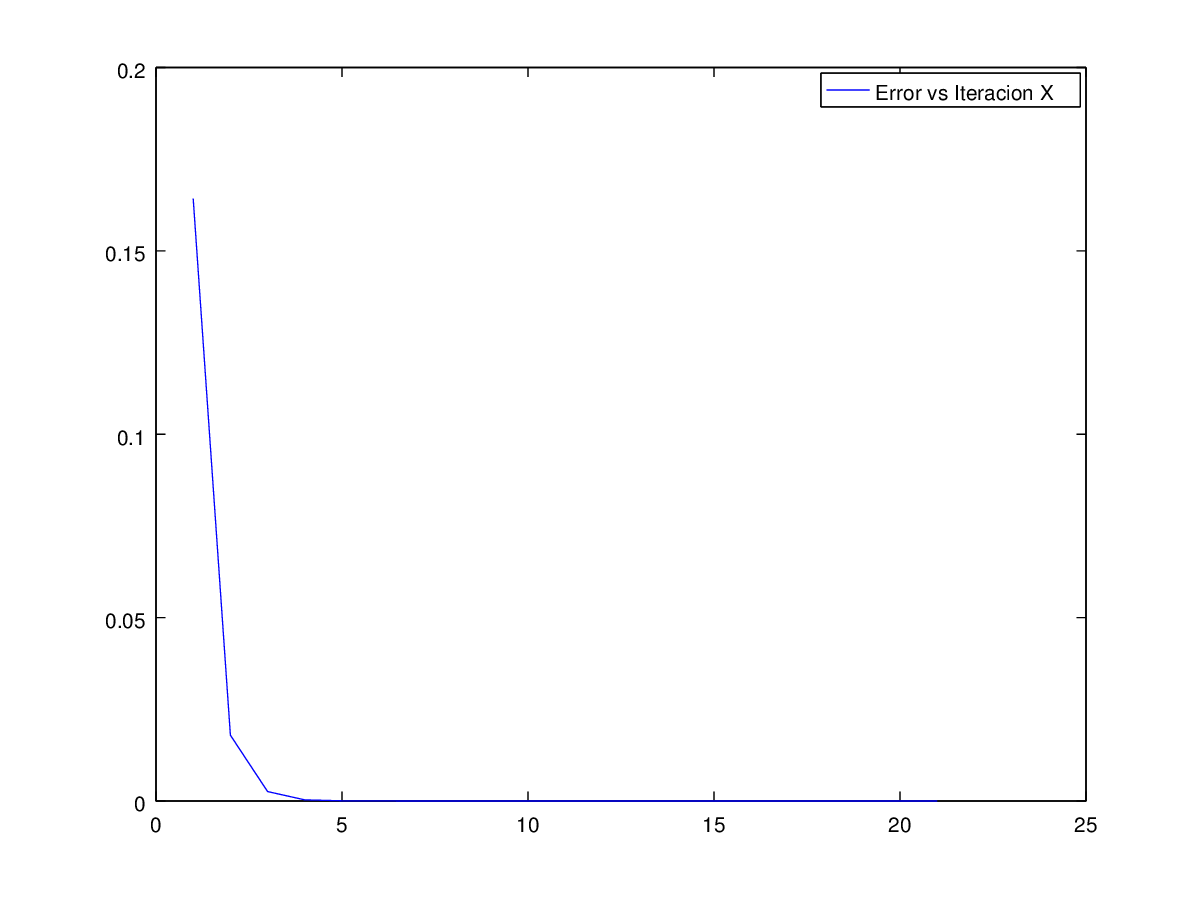
\includegraphics[width=0.7\textwidth]{ErrorVsIteracionPotencia-X.png}
\end{figure}

\begin{figure}[p]
  \caption{Método Arnoldi, Matriz X}
  \centering
    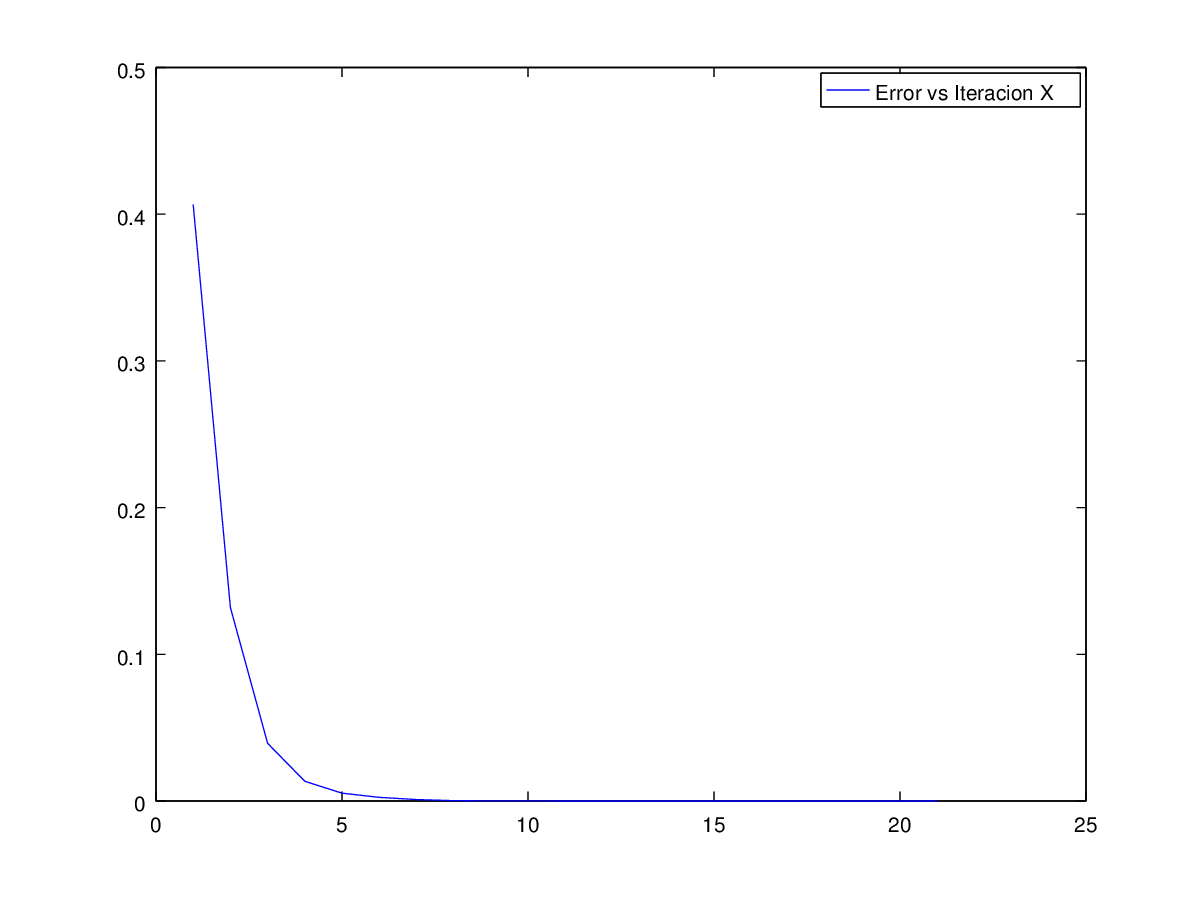
\includegraphics[width=0.7\textwidth]{ErrorVsIteracionArnoldi-X.png}
\end{figure}

\begin{figure}[p]
  \caption{Método Potencias, Matriz Harvard}
  \centering
    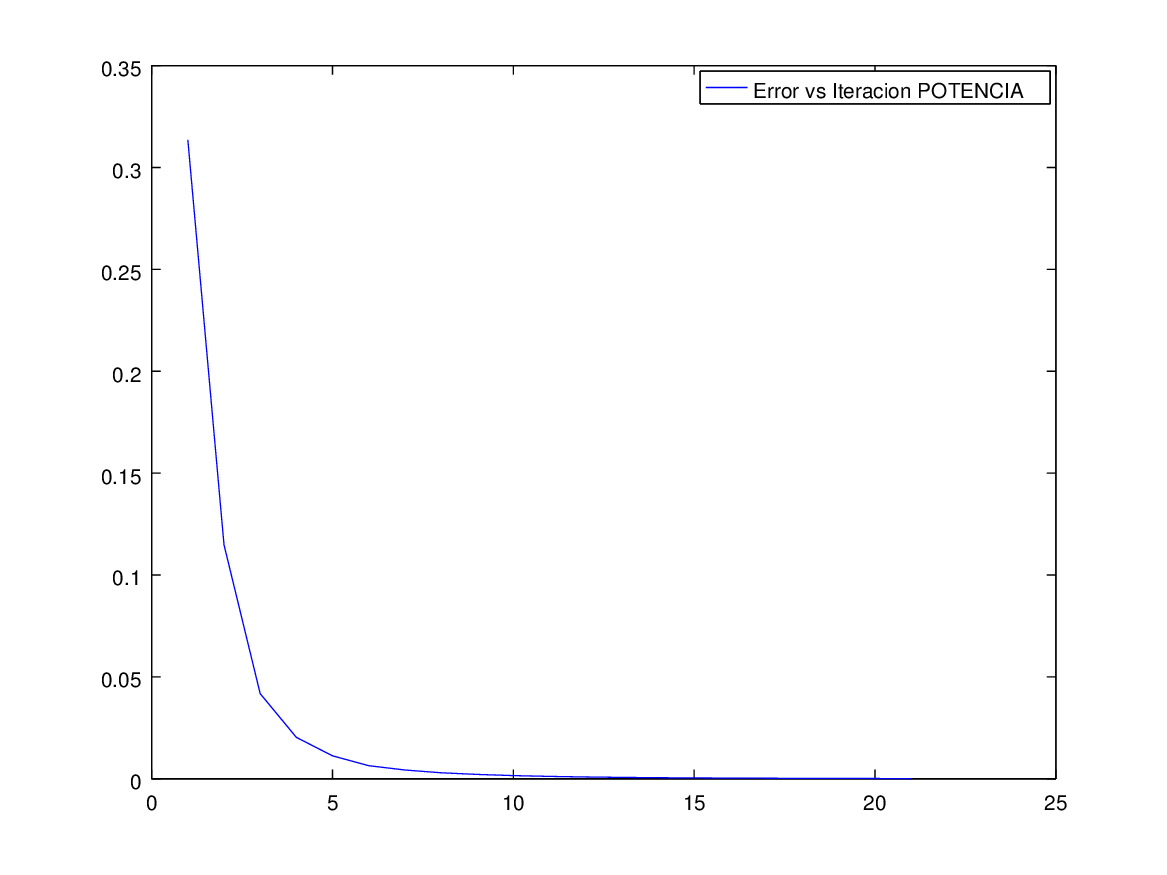
\includegraphics[width=0.7\textwidth]{ErrorVsIteracionPotencia-Harvard.png}
\end{figure}

\begin{figure}[p]
  \caption{Método Arnoldi, Matriz Harvard}
  \centering
    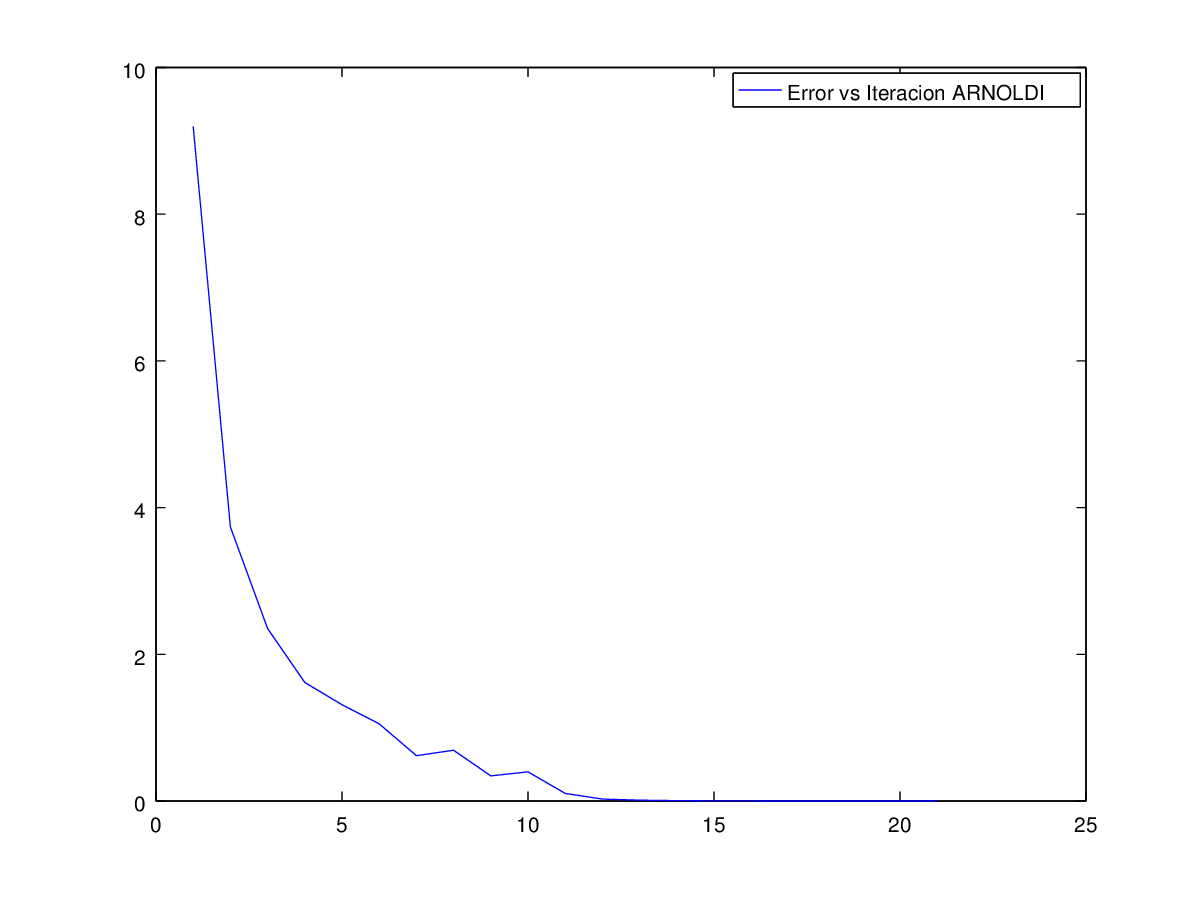
\includegraphics[width=0.7\textwidth]{ErrorVsIteracionArnoldi-Harvard.png}
\end{figure}

\begin{figure}[p]
  \caption{Método Potencias, Matriz Stanford}
  \centering
    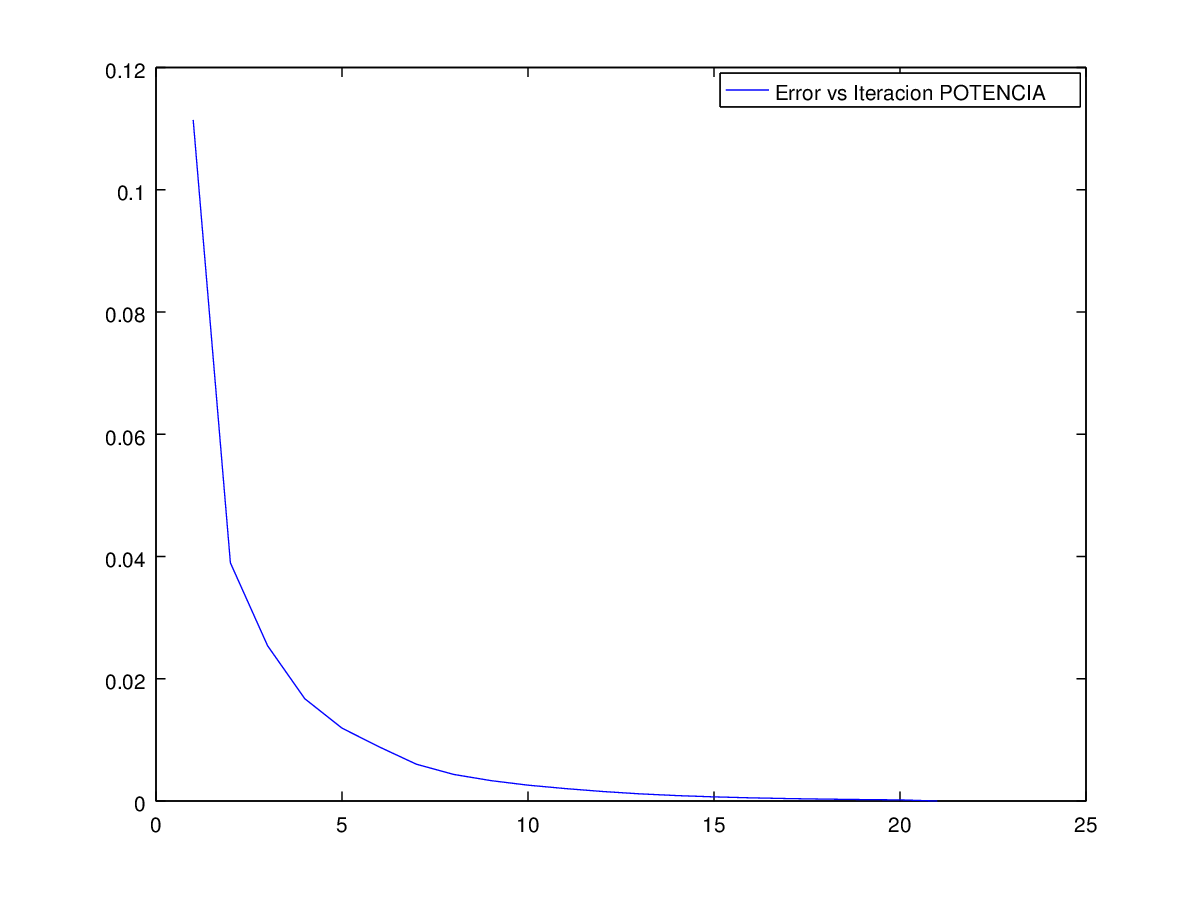
\includegraphics[width=0.7\textwidth]{ErrorVsIteracionPotencia-Stanford.png}
\end{figure}
\begin{figure}[p]
\label{fig:arnoStan}
  \caption{Método Arnoldi, Matriz Stanford}
  \centering
    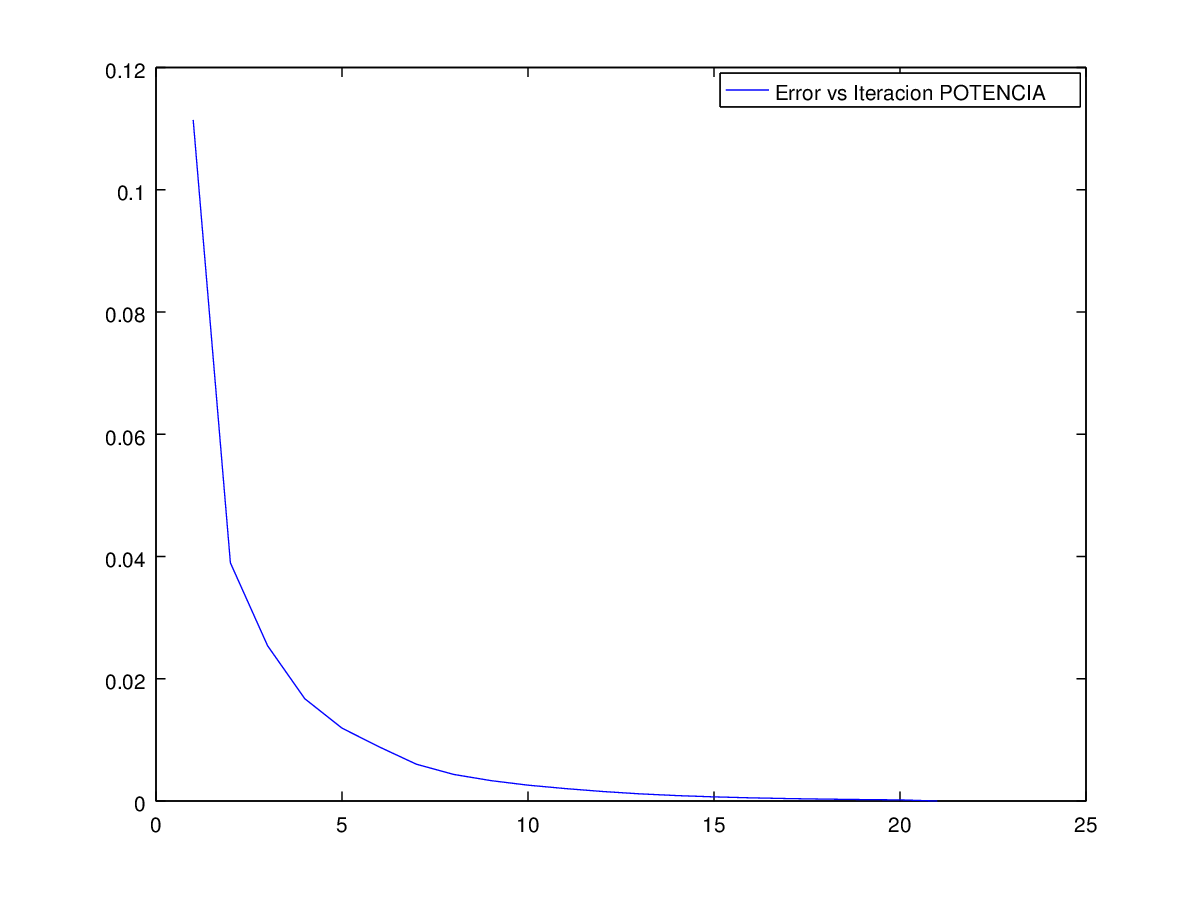
\includegraphics[width=0.7\textwidth]{ErrorVsIteracionPotencia-Stanford.png}
\end{figure}
\begin{figure}[p]
\label{fig:PRHA}
  \caption{Page Rank, Gold Standard, Matriz Harvard}
  \centering
    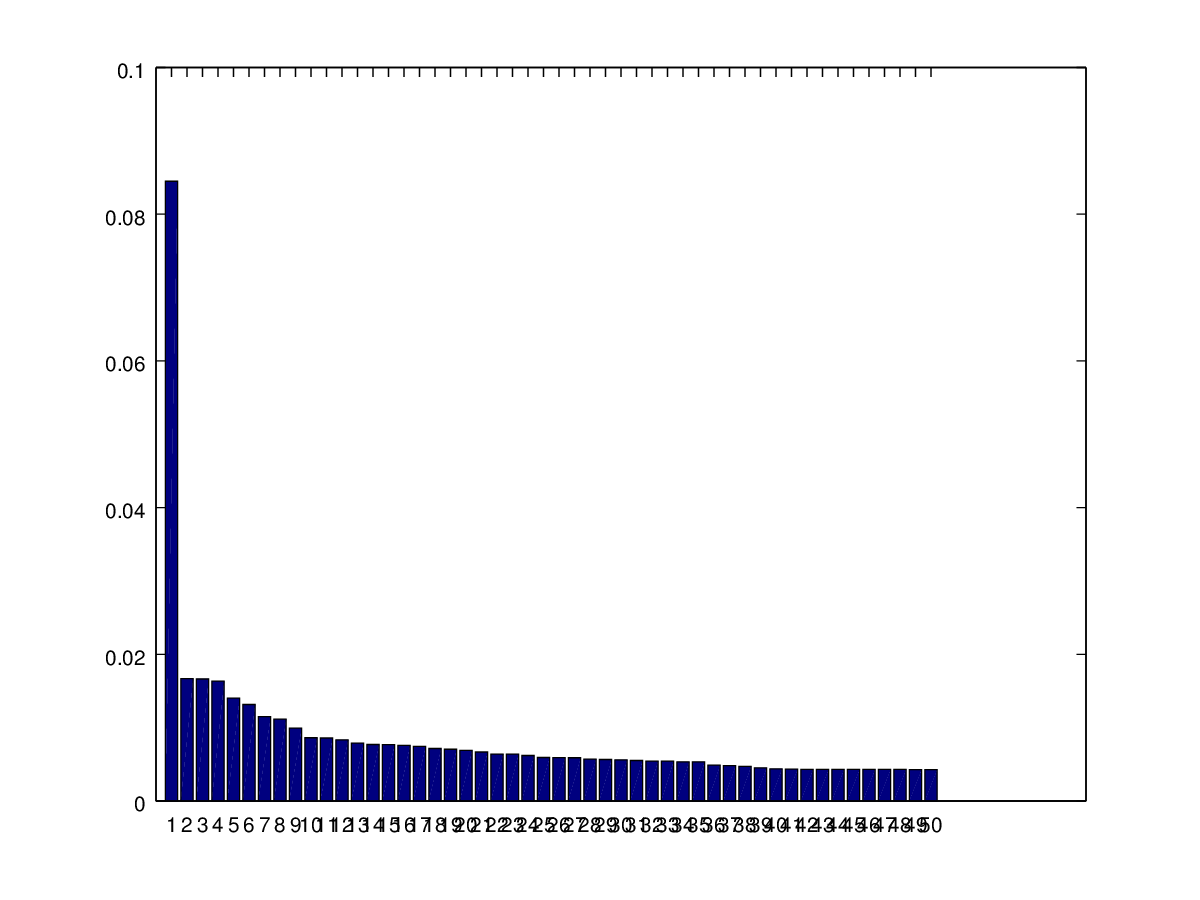
\includegraphics[width=0.7\textwidth]{PageRank-GoldStandard-Harvard.png}
\end{figure}
\begin{figure}[p]
\label{fig:PRST}
  \caption{Page Rank, Gold Standard, Matriz Stanford}
  \centering
    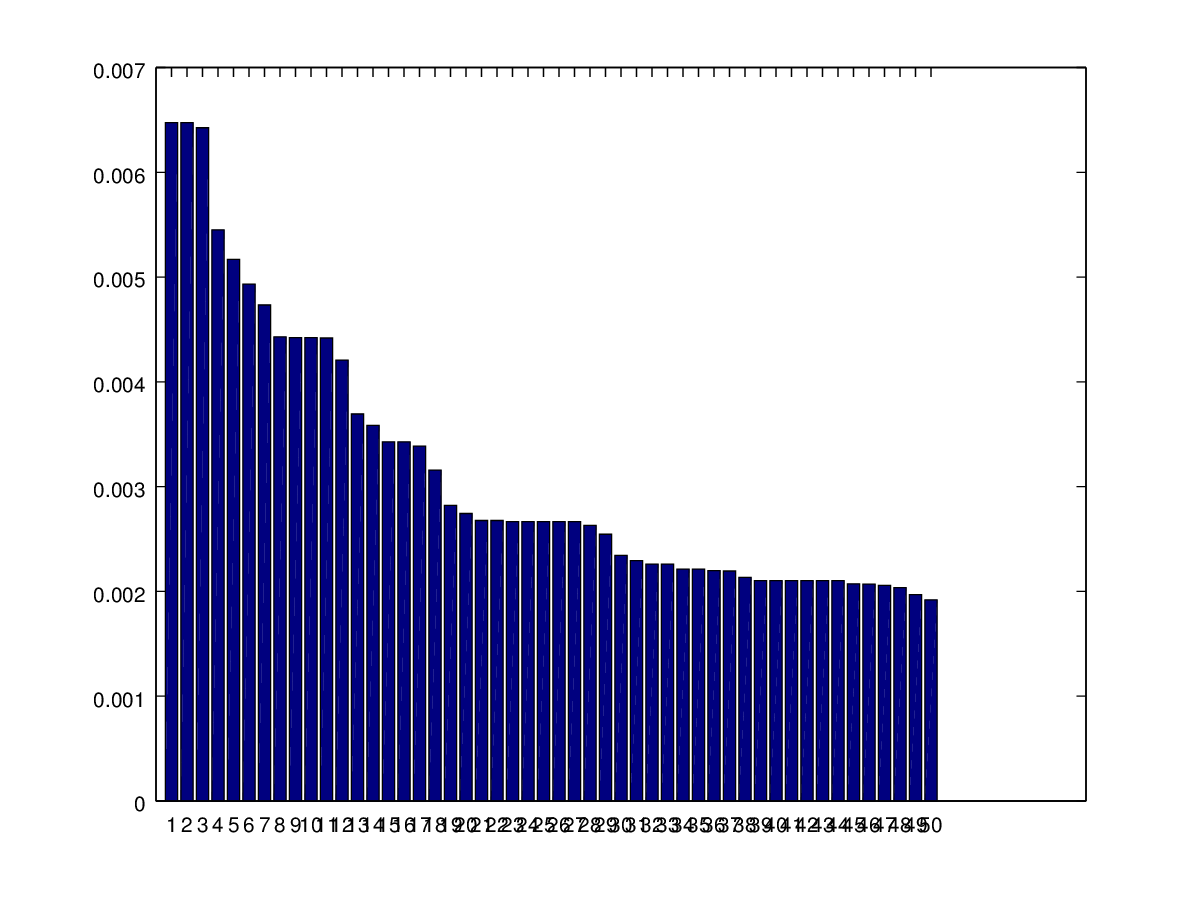
\includegraphics[width=0.7\textwidth]{PageRank-GoldStandard-Stanford.png}
\end{figure}


%----------------------------------------------------------------------------------------
%	SECTION 3
%----------------------------------------------------------------------------------------

\section{Profundización}

\subsection{El segundo valor propio y el problema de Spam}

Si bien el vector propio dominante de la matriz de Google es fundamental ya que representa la distribución estacionaria de la cadena de Markov y por lo tanto indica la probabilidad para un usuario de encontrarse en cada página, los vectores propios asociados al segundo valor propio tiene también importancia según \cite{Sangers2015192} ya que puede ser usado para detectar spam.

\begin{description}
\item[Grafo de la Web]  Se puede ver la Web como un grafo dirigido donde los nodos son las páginas web y los enlaces son los links de una página a otra. Este grafo no es fuertemente conectado. Se dice que el grafo de la web tiene forma de moño: hay tres categorías principales para las páginas web, \textit{IN}, \textit{OUT}, \textit{SCC}. Un usuario puede pasar de una página de \textit{IN} a una de \textit{SCC}, de una de\textit{ SCC} puede pasar a una de \textit{OUT} y puede pasar de una de SCC a otra de SCC, sin embargo no es posible pasar de una de \textit{SCC} a una de \textit{IN}, ni de \textit{OUT} a\textit{ SCC} o a \textit{IN}. Notablemente se ha encontrado que \textit{IN} y \textit{OUT} son de tamaños similares mientras que \textit{SCC} es mucho más grande. La mayoría de las páginas web pertenecen a éstas categorías. \cite{stanfordWebgraph} \cite{Broder2000309}
\end{description}

Se demuestra en \cite{ilprints582} que para toda matriz $A = [cP + (1-c)E]^T$, donde $P$ es una matriz estocastica por filas $nxn$, $E$ es una matriz no negativa $nxn$ de rango 1 estocástica por filas, $0\leq c \leq1$, el segundo vector propio de A tiene módulo $|\lambda_{2}| \leq c $. Más aún si $P$ tiene al menos dos subconjuntos cerrados irreducibles entonces $\lambda_{2} = c$.

Los vectores propios correspondientes al segundo valor propio $\lambda_{2} = c$ son indicadores de certeza en el grafo de la web. En particular cada par de nodos hoja en el grafo SCC para la cadena de Markov P corresponde a un vector propio de A con valor propio $c$. Los nodos hoja en SCC son aquellos subgrafos que pueden tener links entrantes pero no tienen links salientes a otra categoria. Los Spammers utilizan habitualmente dichas estructuras para alterar el PageRank. El análisis de éstas estructuras puede permitir construir estrategias para combatir este tipo de spam.
\cite{ilprints582}


% TODO 


%----------------------------------------------------------------------------------------
%	BIBLIOGRAPHY
%----------------------------------------------------------------------------------------
\newpage

\bibliographystyle{plain}

\bibliography{science}
\newpage

\renewcommand{\appendixname}{Anexos}
\renewcommand{\appendixtocname}{Anexos}
\renewcommand{\appendixpagename}{Anexos}
\begin{appendices}


\lstinputlisting[language=matlab,caption={Potencia.m},label=lst:pot]{Potencia.m}
\newpage
\lstinputlisting[language=matlab,caption={Sistema.m},label=lst:sis]{Sistema.m}
\newpage
\lstinputlisting[language=matlab,caption={PageRankMN.m},label=lst:gs]{PageRankMN.m}
\newpage
\lstinputlisting[language=matlab,caption={Comparacion.m},label=lst:com]{Comparacion.m}
\end{appendices}

%----------------------------------------------------------------------------------------


\end{document}